\section{Systemarchitektur}
Die Architektur des Systems folgt dem bewährten Muster einer \textit{Layered Architecture} (Schichtenarchitektur) \cite{fowler2002}, um eine saubere Trennung der Verantwortlichkeiten (\textit{Separation of Concerns}) zu erzielen. Dies erleichtert nicht nur die Testbarkeit mittels Unit- und Integrationstests, sondern ermöglicht auch zukünftige Erweiterungen ohne das Gesamtsystem neu schreiben zu müssen.

Die Anwendung gliedert sich in vier Hauptschichten:

\begin{figure}[H]
    \centering
    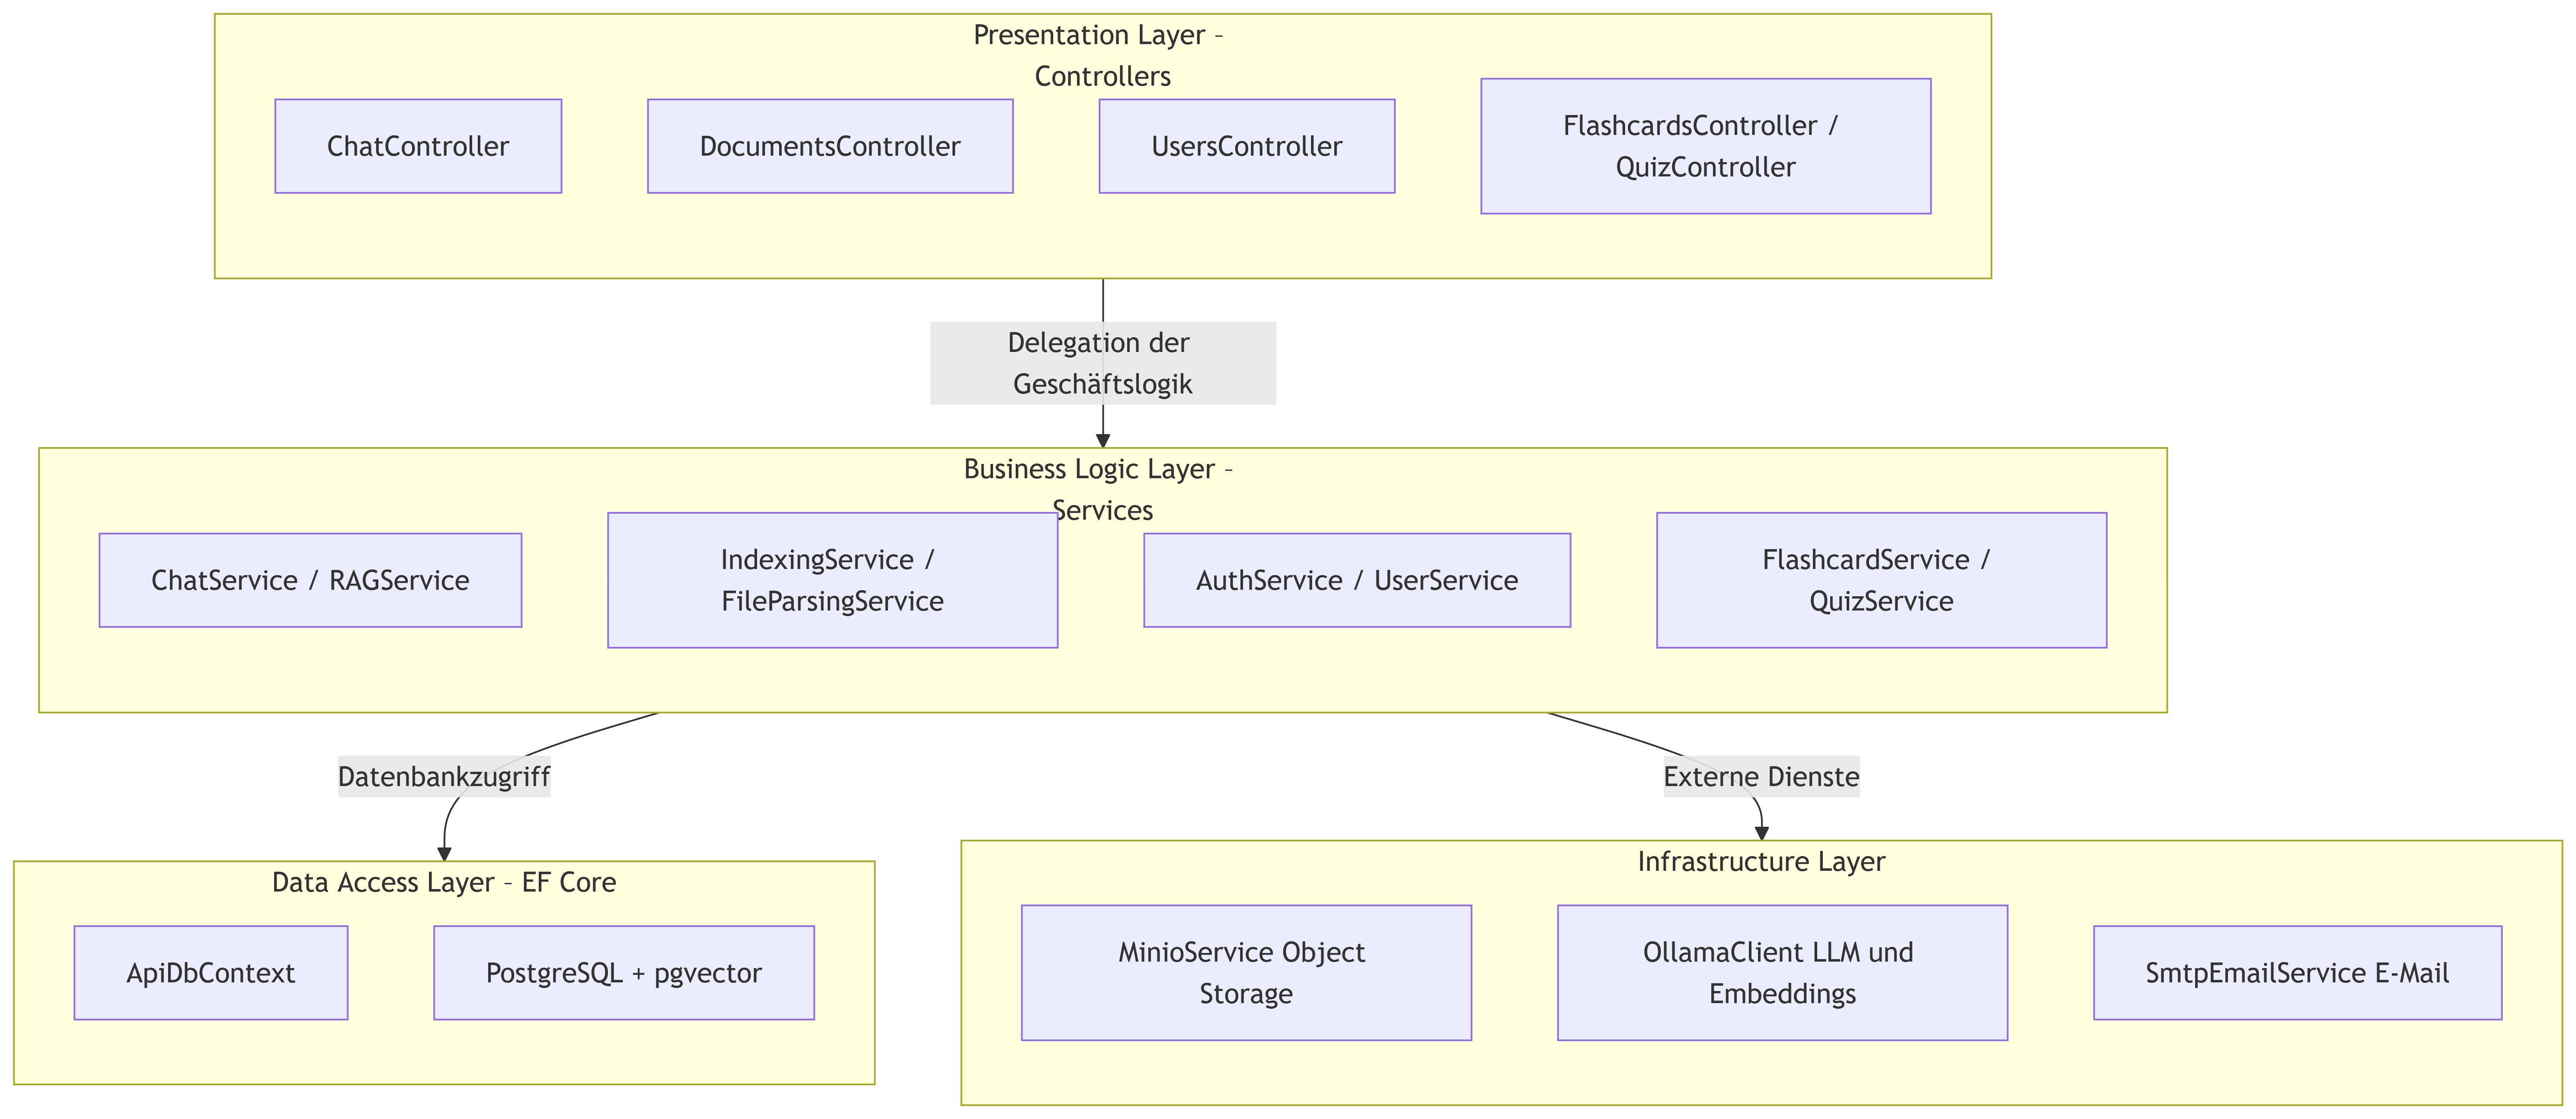
\includegraphics[width=\textwidth]{img/layered_architecture.png}
    \caption{Schichtenarchitektur des EduShelf Backends}
    \label{fig:layered_architecture}
\end{figure}

\subsection{Presentation Layer (Controllers)}
Diese oberste Schicht nimmt HTTP-Anfragen (Requests) entgegen und gibt HTTP-Antworten (Responses) zurück. Sie dient als Tor zur Außenwelt.
\begin{itemize}
    \item \textbf{Verantwortlichkeit:} Routing, Deserialisierung von JSON-Body-Daten, Validierung von Eingaben und Formatierung der Ausgaben.
    \item \textbf{Validierung:} Mithilfe der Bibliothek \textit{FluentValidation} werden eingehende Datenmodelle (DTOs) noch vor der Verarbeitung auf Korrektheit geprüft (z.B. \texttt{UserRegisterValidator}, der sicherstellt, dass E-Mail-Adressen gültig sind und Passwörter Mindestanforderungen erfüllen).
    \item \textbf{Controller:} Die Controller sind schlank gehalten (\textit{Thin Controllers}) und delegieren die eigentliche Geschäftslogik sofort an die Service-Schicht. Beispiel: Der \texttt{ChatController} leitet die Benutzeranfrage direkt an den \texttt{ChatService} weiter.
\end{itemize}

\subsection{Business Logic Layer (Services)}
Hier residiert das \glqq{}Gehirn\grqq{} der Anwendung. Alle Regeln und Prozesse sind in dieser Schicht implementiert.
\begin{itemize}
    \item \textbf{Service-Klassen:} Jeder Bereich hat seinen eigenen Service (z.B. \texttt{AuthService}, \texttt{IndexingService}, \texttt{RAGService}).
    \item \textbf{Orchestrierung:} Services koordinieren den Datenfluss zwischen der Datenbank, externen Diensten (wie MinIO oder Ollama) und der Präsentationsschicht.
    \item \textbf{Dependency Injection:} Alle Services werden über den in .NET integrierte Dependency Injection (DI) Container registriert, was die Austauschbarkeit von Implementierungen zur Laufzeit ermöglicht.
    \item \textbf{Hintergrundverarbeitung:} Für langlaufende Aufgaben wie das Indizieren von Dokumenten wird eine \texttt{BackgroundJobQueue} eingesetzt. Dies entkoppelt rechenintensive Prozesse vom HTTP-Request-Zyklus und verhindert Timeouts im Frontend. Der \texttt{DocumentService} reiht Aufgaben ein, die dann von einem \texttt{BackgroundService} asynchron abgearbeitet werden.
\end{itemize}

\subsection{Data Access Layer (Data)}
Diese Schicht abstrahiert den Zugriff auf die persistente Datenspeicherung.
\begin{itemize}
    \item \textbf{Entity Framework Core (EF Core):} Als Object-Relational Mapper (ORM) \cite{efcore} ermöglicht EF Core die Definition des Datenmodells in C\#-Klassen. SQL-Queries werden zur Laufzeit generiert, was die Entwicklung beschleunigt und vor SQL-Injection schützt.
    \item \textbf{Repositories:} Ebenfalls wird das \texttt{DbContext}-Pattern direkt verwendet, was bei EF Core oft äquivalent zum Repository-Pattern bzw. Unit-of-Work-Pattern ist.
\end{itemize}

\subsection{Infrastructure Layer}
Diese Schicht beinhaltet die technische Anbindung an externe Systeme und Infrastrukturkomponenten.
\begin{itemize}
    \item \textbf{MinIO:} Für die Speicherung unstrukturierter Daten (Blobs) wie PDF-Dokumente oder Bilder.
    \item \textbf{Ollama:} Schnittstelle zum lokalen KI-Modell.
    \item \textbf{E-Mail-Dienst:} Implementierung des \texttt{SmtpEmailService} zum Versenden von Bestätigungs-E-Mails.
\end{itemize}
